\subsection{Belbin}

\begin{figure} [h!]
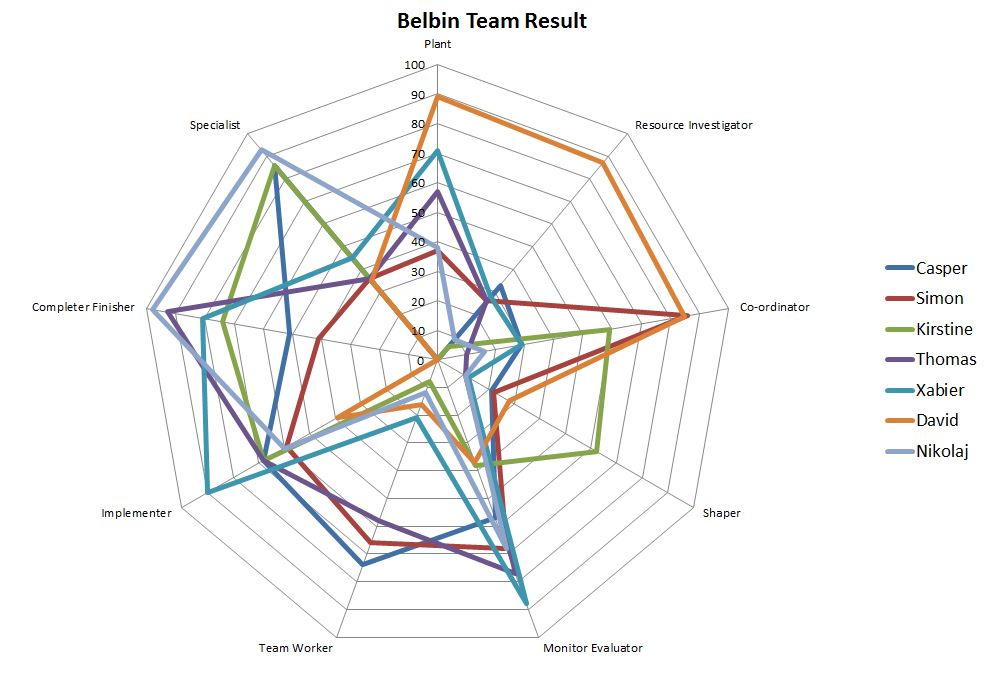
\includegraphics[width=\textwidth]{./graphics/Belbin_spiderweb}
\caption{Belbin Self-perception "Spiderweb"}
\label{belbinspider}
\end{figure}

\begin{table}[h]
\begin{tabular}{|p{0.5\textwidth}|p{0.5\textwidth}|}
\hline
\multicolumn{1}{|c|}{\textit{Contribution:}}                                                  & \multicolumn{1}{c|}{\textit{Allowable Weaknesses:}}                          \\ \hline
\multicolumn{2}{|l|}{\textbf{Top 3 roles:}}                                                                                                                                  \\ \hline
\multicolumn{2}{|c|}{\textbf{Monitor Evaluator}}                                                                                                                             \\ \hline
Sober, strategic and discerning. Sees all options and judges accurately.                      & Lacks drive and ability to inspire others. Can be overly critical to others. \\ \hline
\multicolumn{2}{|c|}{\textbf{Implementer}}                                                                                                                                   \\ \hline
Practical, reliable, efficient. Turns ideas into actions and organizes work that needs tobe done.& Somewhatinflexible. Slow to respond to new possibilities.                  \\ \hline
\multicolumn{2}{|c|}{\textbf{Completer Finisher}}                                                                                                                            \\ \hline
Painstaking, conscientious, anxious. Searches out errors. Polishes and perfects.              & Inclined to worry unduly. Reluctant to delegate.                             \\ \hline
\multicolumn{2}{|l|}{\textbf{Worst 3 Roles:}}                                                                                                                                \\ \hline
\multicolumn{2}{|c|}{\textbf{Shaper}}                                                                                                                                        \\ \hline
Challenging, dynamic, thrives on pressure. Has the drive and courage to overcome obstacles. & Prone to provocation. Offends people’s feelings.                             \\ \hline
\multicolumn{2}{|c|}{\textbf{Plant}}                                                                                                                                         \\ \hline
Creative, imaginative, free-thinking. Generates ideas and solves difficult problems.        & Ignores incidentals. Too preoccupied to communicate effectively.             \\ \hline
\multicolumn{2}{|c|}{\textbf{Resource Investigator}}                                                                                                                         \\ \hline
Outgoing, enthusiastic, communicative. Explores opportunities and develops contacts.        & Over-optimistic. Loses interest once initial enthusiasm has passed.          \\ \hline
\end{tabular}
\caption{Top/Worst 3 Belbin Self-perception for the group}
\label{belbintable}
\end{table}

This table (table \ref{belbintable}) is based on the results of the individual tests, which is also reflected by the spider web chart (figure \ref{belbinspider}). The table shows the strong and weak roles for the team profiles.

It is very clear that the group has a major potential when it comes to developing solutions to perfection, while being able to investigate the different possibilities. This could be explained by the amount of specialists in the group.

It is also very clear that the group lacks drive and a key person to set the pace of the work processes. The group has to be aware that the beginning of project is the vulnerable timespan. This is due to the missing Plants who provide creativity and innovation to the group, together with the resource investigators who makes sure the actual ideas are possible at all.
 
%Since we already encountered difficulties in the beginning of the project, it is obvious that the group is missing ideas to work with. That could also explain why we decided to go with the basic idea that was described in the project introduction papers.

%The strengths and weaknesses can all be related to the group-SWOT test.

%<Insert comparison>.